\documentclass{beamer}

\usepackage{comment}
\usepackage{color}
\usepackage{listings}
\usepackage{verbatim}
\usepackage{multicol}
\usepackage{booktabs}
\usepackage{textpos}
\usepackage{graphicx}
\usepackage{graphics}
\definecolor{green}{RGB}{0,128,0}

\def\EQ#1\EN{\begin{equation*}#1\end{equation*}}
\def\BA#1\EA{\begin{align*}#1\end{align*}}
\def\BS#1\ES{\begin{split*}#1\end{split*}}
\newcommand{\bc}{\begin{center}}
\newcommand{\ec}{\end{center}}
\newcommand{\eq}{\ =\ }
\newcommand{\degc}{$^\circ$C}

\def\p{\partial}
\def\qbs{\boldsymbol{q}}
\def\Dbs{\boldsymbol{D}}
\def\A{\mathcal A}
\def\gC{\mathcal C}
\def\gD{\mathcal D}
\def\gL{\mathcal L}
\def\M{\mathcal M}
\def\P{\mathcal P}
\def\Q{\mathcal Q}
\def\gR{\mathcal R}
\def\gS{\mathcal S}
\def\X{\mathcal X}
\def\bnabla{\boldsymbol{\nabla}}
\def\bnu{\boldsymbol{\nu}}
\renewcommand{\a}{{\alpha}}
%\renewcommand{\a}{{}}
\newcommand{\s}{{\sigma}}
\newcommand{\bq}{\boldsymbol{q}}
\newcommand{\bz}{\boldsymbol{z}}
\def\bPsi{\boldsymbol{\Psi}}

\def\Li{\textit{L}}
\def\Fb{\textbf{f}}
\def\Jb{\textbf{J}}
\def\cb{\textbf{c}}

\def\Dt{\Delta t}
\def\tpdt{{t + \Delta t}}
\def\bpsi{\boldsymbol{\psi}}
\def\dbpsi{\delta \boldsymbol{\psi}}
\def\bc{\textbf{c}}
\def\dbc{\delta \textbf{c}}
\def\arrows{\rightleftharpoons}

\newcommand{\bGamma}{\boldsymbol{\Gamma}}
\newcommand{\bOmega}{\boldsymbol{\Omega}}
%\newcommand{\bPsi}{\boldsymbol{\Psi}}
%\newcommand{\bpsi}{\boldsymbol{\psi}}
\newcommand{\bO}{\boldsymbol{O}}
%\newcommand{\bnu}{\boldsymbol{\nu}}
\newcommand{\bdS}{\boldsymbol{dS}}
\newcommand{\bg}{\boldsymbol{g}}
\newcommand{\bk}{\boldsymbol{k}}
%\newcommand{\bq}{\boldsymbol{q}}
\newcommand{\br}{\boldsymbol{r}}
\newcommand{\bR}{\boldsymbol{R}}
\newcommand{\bS}{\boldsymbol{S}}
\newcommand{\bu}{\boldsymbol{u}}
\newcommand{\bv}{\boldsymbol{v}}
%\newcommand{\bz}{\boldsymbol{z}}
\newcommand{\pressure}{P}

\def\water{H$_2$O}
\def\calcium{Ca$^{2+}$}
\def\copper{Cu$^{2+}$}
\def\magnesium{Mg$^{2+}$}
\def\sodium{Na$^+$}
\def\potassium{K$^+$}
\def\uranium{UO$_2^{2+}$}
\def\hion{H$^+$}
\def\hydroxide{0H$^-$}
\def\bicarbonate{HCO$_3^-$}
\def\carbonate{CO$_3^{2-}$}
\def\cotwo{CO$_2$(aq)}
\def\chloride{Cl$^-$}
\def\fluoride{F$^-$}
\def\phosphoricacid{HPO$_4^{2-}$}
\def\nitrate{NO$_3^-$}
\def\sulfate{SO$_4^{2-}$}
\def\souotwooh{$>$SOUO$_2$OH}
\def\sohuotwocothree{$>$SOHUO$_2$CO$_3$}
\def\soh{$>$SOH}

\newcommand\gehcomment[1]{{{\color{orange} #1}}}
\newcommand\add[1]{{{\color{blue} #1}}}
\newcommand\remove[1]{\sout{{\color{red} #1}}}
\newcommand\codecomment[1]{{{\color{green} #1}}}
\newcommand\redcomment[1]{{{\color{red} #1}}}
\newcommand\bluecomment[1]{{{\color{blue} #1}}}
\newcommand\greencomment[1]{{{\color{green} #1}}}
\newcommand\magentacomment[1]{{{\color{magenta} #1}}}

\begin{comment}
\tiny
\scriptsize
\footnotesize
\small
\normalsize
\large
\Large
\LARGE
\huge
\Huge
\end{comment}

\begin{document}
\title{1D Calcite Scenario\ldots in a Nutshell}
\author{Glenn Hammond}
\date{\today}

%\frame{\titlepage}

%-----------------------------------------------------------------------------
\section{Description of 1D Variables Saturated Flow Scenarios}

\subsection{1D Variably Saturated Flow Conceptual Model}

\frame{\frametitle{Description of 1D Variably Saturated Flow Scenario}
The ``1D Variably Saturated Flow Scenario'' simulates single phase groundwater flow within the vadose and saturated zones in a vertical column measuring 10 meters in height with unit cross sectional area.  Assumptions with regard to flow include:
\begin{itemize}
  \small
  \item Problem domain: $1 \times 1 \times 10$ m (x $\times$ y $\times$ z)
  \item Grid resolution $1 \times 1 \times 0.1$ m
  \item Water table at z = 1 m
  \item Recharge of 10 cm/y at top of surface
  \item Material properties
  \begin{itemize}
    \footnotesize
    \item $k \eq 10^{-12}$ [m$^2$]
    \item $\varphi \eq 0.25$
    \item Saturation function: van Genutchen
    \begin{itemize}
      \scriptsize
      \item $\alpha \eq 10^{-4}$ [Pa$^{-1}$]
      \item $m \eq 0.5$
      \item $s_r \eq 0.1$
    \end{itemize}
    \item Permeability function: Mualem
  \end{itemize}
  \item Total simulation time: 10 y
\end{itemize}
\begin{textblock}{.5}[1,1](9.5,-.75)
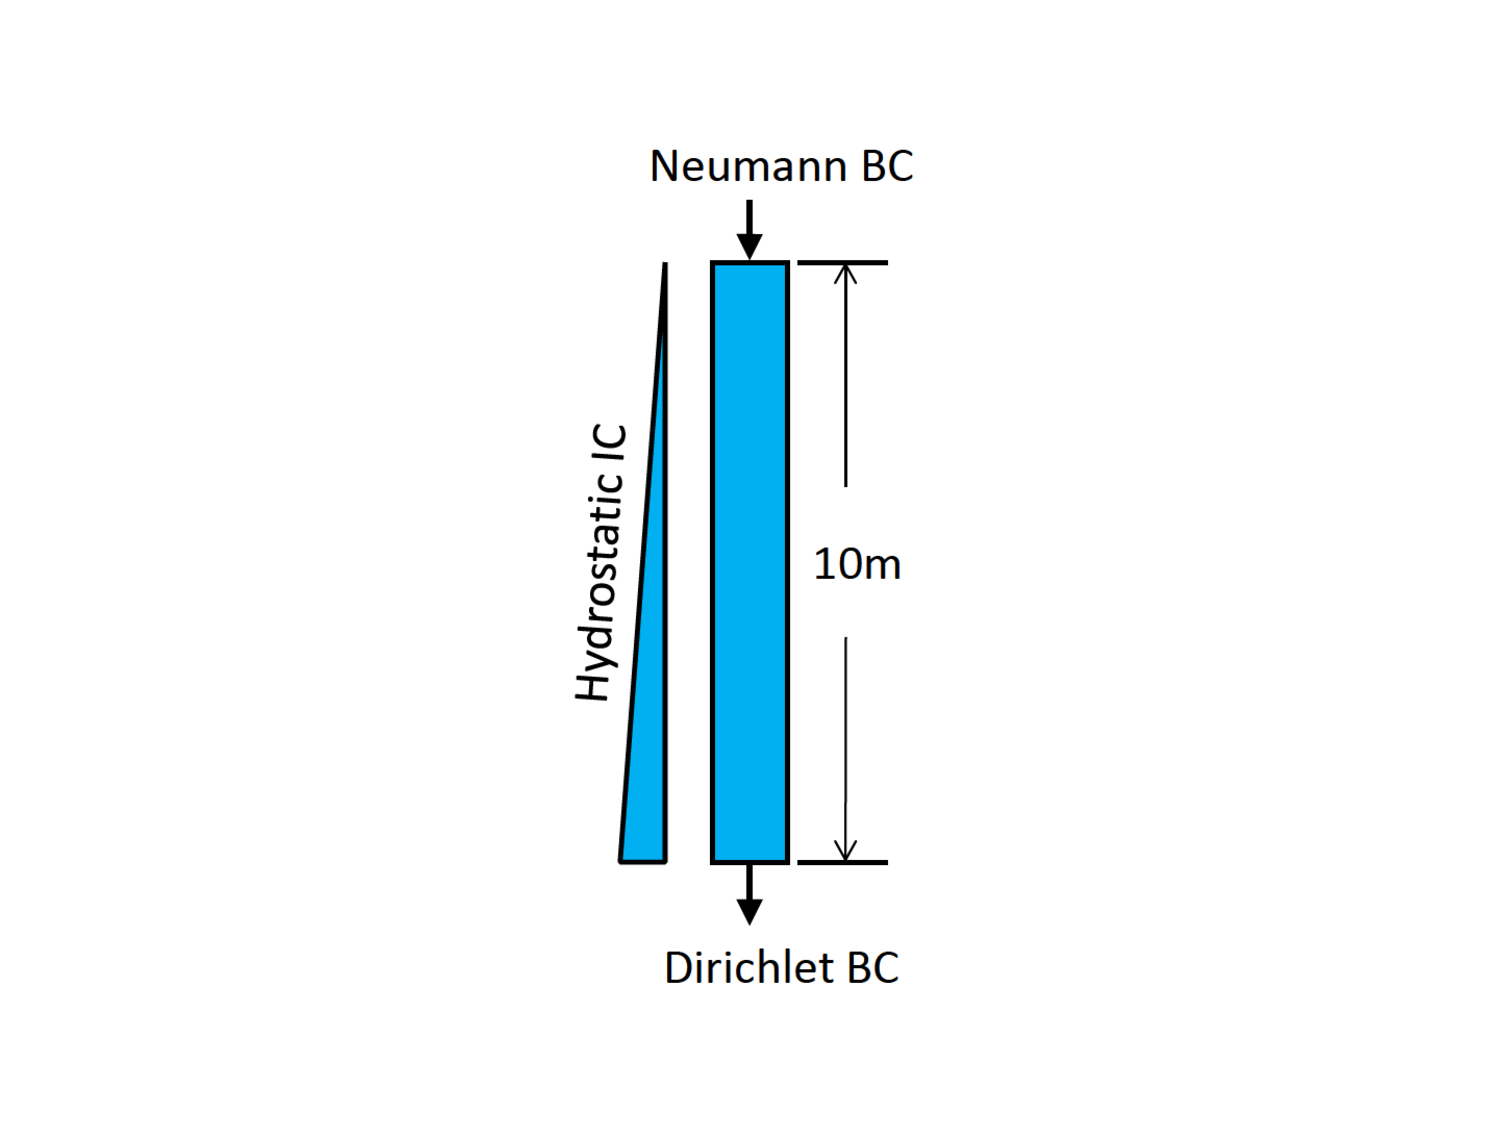
\includegraphics[height=2in]{./vsat_flow_uniform}
\end{textblock}  
}

%-----------------------------------------------------------------------------
\subsection{Governing Equations}

\frame{\frametitle{Governing Flow Equations: Richards Equation}

{\bf Continuity Equation:}
\EQ
\frac{\p}{\p t} \big(\varphi s \rho\big) + \bnabla\cdot\rho\bq \eq Q
\EN


{\bf Darcy's Law:}
\EQ
\bq \eq -\frac{\bk k_r}{\mu} \bnabla\big(\pressure-\rho g z\big)
\EN

\normalsize

\begin{columns}[c]
  \column{0.5\linewidth}
  \begin{itemize}
    \item $\varphi \eq $ porosity
    \item $s \eq $ saturation
    \item $\rho \eq $ water density
    \item $\bk \eq $ intrinsic permeability tensor
    \item $k_r \eq $ relative permeability
  \end{itemize}
  \column{0.5\linewidth}
  \begin{itemize}
    \item $\mu \eq $ viscosity
    \item $\pressure \eq $ water pressure
    \item $g \eq $ gravity
    \item $z \eq $ distance in direction of gravity
    \item[]
  \end{itemize}
\end{columns}


}

%-----------------------------------------------------------------------------
\frame{\frametitle{Constitutive Relations}

\begin{itemize}
  \item Capillary Pressure Relations
  \begin{itemize}
    \item van Genuchten
    \begin{itemize}
      \item Effective Saturation:
      \EQ\label{seff}
      s_e \eq \left[1+\left( \alpha |P_c| \right)^n \right]^{-m}\nonumber
      \EN
      \item Saturation:
      \EQ
      s \eq s_e (1-s_r)+s_r
      \EN
    \end{itemize}
  \end{itemize}
  \item Permeability Function Relations
  \begin{itemize}
    \item Mualem
    \EQ\label{krl}
    k_r \eq \sqrt{s_e} \left\{1-\left[1-s_e^{1/m} \right]^m \right\}^2\nonumber
    \EN
  \end{itemize}
\end{itemize}

\bigskip
\footnotesize
\begin{columns}[c]
  \column{0.6\linewidth}
  \begin{itemize}
    \item $s \eq $ saturation
    \item $s_e \eq $effective saturation
    \item $s_r \eq $ residual saturation
  \item $P_c \eq $ capillary pressure $\eq P_\text{atm} - \pressure$
  \end{itemize}
  \column{0.4\linewidth}
  \begin{itemize}
    \item $\alpha \eq $ van Genuchten function parameter $\alpha$
    \item $n \eq $ van Genuchten $n$
    \item $m \eq $ van Genuchten  $\eq 1 - 1/n$
  \end{itemize}
\end{columns}

}

%-----------------------------------------------------------------------------
\section{Description of Input Deck}

%-----------------------------------------------------------------------------
\subsection{SIMULATION}

\begin{frame}[fragile]\frametitle{SIMULATION}

\begin{itemize}
\item Specify Richards flow mode
\end{itemize}


\begin{semiverbatim}

SIMULATION
  SIMULATION_TYPE SUBSURFACE
  PROCESS_MODELS
    SUBSURFACE_FLOW flow
      MODE RICHARDS
    /
  /
END

SUBSURFACE
 ...
END_SUBSURFACE
\end{semiverbatim}

\end{frame}

%-----------------------------------------------------------------------------
\subsection{GRID}
\begin{frame}[fragile,containsverbatim]\frametitle{GRID}

\begin{itemize}
  \item Problem domain: $1 \times 1 \times 10$ m (x $\times$ y $\times$ z)
  \item Grid resolution $1 \times 1 \times 0.1$ m
\end{itemize}

\begin{semiverbatim}
GRID
  TYPE STRUCTURED        \bluecomment{! structured grid}
  NXYZ 1 1 100           \bluecomment{! NX, NY, NZ}
  BOUNDS             \bluecomment{! define the rectangular domain}
    0.d0 0.d0 0.d0   \bluecomment{! xmin ymin zmin}
    1.d0 1.d0 10.d0  \bluecomment{! xmax ymax zmax}
  /  \bluecomment{! <-- closes out BOUNDS card}
END  \bluecomment{! <-- closes out GRID card}
\end{semiverbatim}

\end{frame}

%-----------------------------------------------------------------------------
\subsection{REGION}

\begin{frame}[fragile,containsverbatim,allowframebreaks]\frametitle{REGION}

\begin{itemize}
  \item Delineate regions in the 1D domain for:
  \begin{itemize}
    \item top boundary face
    \item bottom boundary face
    \item entire domain (all)
  \end{itemize}
\end{itemize}

\begin{semiverbatim}
REGION all            \bluecomment{! define a region and name it: \greencomment{all}}
  COORDINATES         \bluecomment{! using \redcomment{volumetric} coordinates}
    0.d0 0.d0 0.d0    \bluecomment{! lower coordinate: xmin ymin zmin}
    1.d0 1.d0 10.d0   \bluecomment{! upper coordinate: xmax ymax zmax}
  /   \bluecomment{! <-- closes out COORDINATES card}
END   \bluecomment{! <-- closes out REGION card}

\newpage
REGION top            \bluecomment{! define region:} \greencomment{top}
  FACE TOP            \bluecomment{! define the face of the grid cell}
  COORDINATES         \bluecomment{! using \redcomment{surface} coordinates}
    0.d0 0.d0 10.d0
    1.d0 1.d0 10.d0
  /
END

REGION bottom         \bluecomment{! define region:} \greencomment{bottom}
  FACE BOTTOM         \redcomment{! WEST, EAST, SOUTH, NORTH,}
  COORDINATES         \redcomment{!   BOTTOM, TOP} \bluecomment{ are keywords}
    0.d0 0.d0 0.d0    \bluecomment{!   in PFLOTRAN.}
    1.d0 1.d0 0.d0
  /
END

\end{semiverbatim}

\end{frame}

%-----------------------------------------------------------------------------
\subsection{MATERIAL\_PROPERTY}

\begin{frame}[fragile,containsverbatim]\frametitle{MATERIAL\_PROPERTY}

\begin{itemize}
  \item Define a soil with :
  \begin{itemize}
    \item Material id = 1
    \item Porosity = 0.25
    \item Permeability = 1 Darcy ($10^{-12}$ m$^2$)
  \end{itemize}
\end{itemize}

\begin{semiverbatim}
MATERIAL_PROPERTY soil1  \bluecomment{! define a material:} \greencomment{soil1}
  ID 1             \bluecomment{! material ID assigned to grid cells}
  POROSITY 0.25d0
  PERMEABILITY     \bluecomment{! permeability is defined in a block}
    PERM_ISO 1.d-12  \bluecomment{! isotropic permeability}
  /
  CHARACTERISTIC\_CURVES cc1 \bluecomment{! couple the characteristic}
END                         \bluecomment{!   curve}
\end{semiverbatim}

\end{frame}

%-----------------------------------------------------------------------------
\subsection{CHARACTERISTIC\_CURVES}

\begin{frame}[fragile]\frametitle{CHARACTERISTIC\_CURVES}

\begin{itemize}
\item Set van Genuchten parameters
\item Assume Mualem permeability (default)
\end{itemize}

\begin{semiverbatim}
CHARACTERISTIC_CURVES cc1
  SATURATION_FUNCTION VAN_GENUCHTEN
    ALPHA  1.d-4   \bluecomment{! [Pa^-1]}
    M 0.5d0        \bluecomment{! van Genuchten m in n = 1/(1-m)}
    LIQUID_RESIDUAL_SATURATION 0.1d0
  /
  PERMEABILITY_FUNCTION MUALEM_VG_LIQ
    M 0.5d0
    LIQUID_RESIDUAL_SATURATION 0.1d0
  /
END
\end{semiverbatim}

\end{frame}

%-----------------------------------------------------------------------------
\subsection{STRATA}

\begin{frame}[fragile]\frametitle{STRATA}

\begin{itemize}
\item Couple \greencomment{soil1} rock/soil type with region \greencomment{all} to define a stratigraphic unit
\end{itemize}

\begin{semiverbatim}

STRATA
  REGION all
  MATERIAL soil1
END


\end{semiverbatim}

\end{frame}

%-----------------------------------------------------------------------------
\subsection{FLOW\_CONDITION}

\begin{frame}[fragile]\frametitle{FLOW\_CONDITION}

\begin{itemize}
\item Specify an initial hydrostatic pressure
\item Specify a boundary flux at top of domain
\end{itemize}

\begin{semiverbatim}
FLOW_CONDITION initial_pressure \bluecomment{! named \greencomment{initial_pressure}}
  TYPE
    PRESSURE HYDROSTATIC \bluecomment{! type is \redcomment{hydrostatic}}
  /                      \bluecomment{!   for pressure}
  DATUM 0.d0 0.d0 1.d0   \bluecomment{! water table at 1 m}
  PRESSURE 101325.d0     \bluecomment{! pressure set to atmospheric}
END                      \bluecomment{!   at water table}

FLOW_CONDITION recharge  \bluecomment{! named \greencomment{recharge}}
  TYPE
    FLUX NEUMANN         \bluecomment{! type is \redcomment{neumann} for a flux}
  /
  FLUX 10.d0 cm/y        \bluecomment{! Darcy velocity of 10 cm/y}
END
\end{semiverbatim}

\end{frame}

%-----------------------------------------------------------------------------
\subsection{INITIAL\_CONDITION}

\begin{frame}[fragile]\frametitle{INITIAL\_CONDITION}

\begin{itemize}
\item Couple the \greencomment{initial\_pressure} flow condition with region \greencomment{all} for the initial condition
\end{itemize}

\begin{semiverbatim}

INITIAL_CONDITION           \bluecomment{! notice no name}
  FLOW_CONDITION initial_pressure
  REGION all
END

\end{semiverbatim}

\end{frame}

%-----------------------------------------------------------------------------
\subsection{BOUNDARY\_CONDITION}

\begin{frame}[fragile]\frametitle{BOUNDARY\_CONDITION}

\begin{itemize}
\item Couple the \greencomment{inlet} flow condition with region \greencomment{top} for the \redcomment{inlet} boundary condition.
\item Couple the \greencomment{initial\_pressure} flow condition with region \greencomment{bottom} for the \redcomment{outlet} boundary condition.
\end{itemize}

\begin{semiverbatim}

BOUNDARY_CONDITION outlet          \bluecomment{! name is optional,}
  FLOW_CONDITION initial_pressure  \bluecomment{!   but recommended}
  REGION bottom
END

BOUNDARY_CONDITION inlet
  FLOW_CONDITION recharge
  REGION top
END

\end{semiverbatim}

\end{frame}

%-----------------------------------------------------------------------------
\subsection{LINEAR\_SOLVER}

\begin{frame}[fragile]\frametitle{LINEAR\_SOLVER}

\begin{itemize}
\item Due to the small problem size, request a direct solver.
\item PETSc provides a direct solve through LU matrix factorization as a preconditioner with no outer Krylov solve.
\end{itemize}

\begin{semiverbatim}

LINEAR_SOLVER FLOW     \bluecomment{! flow solver}
  SOLVER DIRECT        \bluecomment{! sets both the below}
END

\bluecomment{! could also use:}
LINEAR_SOLVER FLOW
  KSP_TYPE PREONLY     \bluecomment{! turn off Krylov solver}
  PC_TYPE PCLU         \bluecomment{! turn on LU preconditioner}
END

\end{semiverbatim}

\end{frame}

%-----------------------------------------------------------------------------
\subsection{TIME}

\begin{frame}[fragile]\frametitle{TIME}

\begin{itemize}
\item Set final simulation time to 10 years
\item Set initial time step size to 1 hour
\item Set maximum time step size to 0.05 years
\end{itemize}


\begin{semiverbatim}

TIME
  FINAL_TIME 10.d0 \redcomment{y}            \bluecomment{! within TIME, time units}
  INITIAL_TIMESTEP_SIZE 1.d0 \redcomment{h}  \bluecomment{!   are recognized and}
  MAXIMUM_TIMESTEP_SIZE 5.d-2 \redcomment{y} \bluecomment{!   converted to SI}
END                             \bluecomment{! (i.e. \redcomment{y}, \redcomment{h} --> \greencomment{s}).}
\end{semiverbatim}

\end{frame}

%-----------------------------------------------------------------------------
\subsection{OUTPUT}

\begin{frame}[fragile]\frametitle{OUTPUT}

\begin{itemize}
\item Specify output times (0.01, 0.1, 1.) and format (Tecplot point datapacking).
\item The initial and final simulation times are automatically added to the list of output times.
\end{itemize}


\begin{semiverbatim}

OUTPUT
  TIMES \redcomment{y} 0.01 0.1 1.     \bluecomment{! within OUTPUT, time units}
  FORMAT TECPLOT POINT    \bluecomment{!   are recognized and}
END                       \bluecomment{!   converted to SI}
                          \bluecomment{!   (i.e. \redcomment{y} --> \greencomment{s}).}
\end{semiverbatim}

\end{frame}

%-----------------------------------------------------------------------------
\subsection{Running vsat_flow.in}

\begin{frame}[fragile]\frametitle{Running PFLOTRAN}

\begin{semiverbatim}

> cd $PFLOTRAN_DIR
> cd shortcourse/exercises/1D_variably_saturated_flow
> pflotran -input_prefix vsat_flow
> python vsat_flow.py
\end{semiverbatim}

\end{frame}

%-----------------------------------------------------------------------------
\section{Description of Input Deck: Adding a pulsed recharge}

\subsection{Input File Modifications}

\begin{frame}[fragile]\frametitle{Adding pulsed recharge over first 0.2 years}


Input File Modifications
\begin{itemize}
\item Modify cards:
  \begin{itemize}
    \item FLOW\_CONDITION
    \item TIMES
   \end{itemize}
\end{itemize}

\end{frame}

%-----------------------------------------------------------------------------
\subsection{FLOW\_CONDITION}

\begin{frame}[fragile]\frametitle{FLOW\_CONDITION}

\begin{itemize}
\item Replace the constant flux with a pulsed flux of 100 cm/y over the first 0.2 years.
\end{itemize}


\begin{semiverbatim}

FLOW_CONDITION recharge
  TYPE
    FLUX NEUMANN
  /
  \magentacomment{#}FLUX 10.d0 cm/y   \bluecomment{! comment out constant value}
  \magentacomment{FLUX LIST          \bluecomment{! flux is now a transient dataset}
    TIME_UNITS y     \bluecomment{! units of time value: \redcomment{year}}
    DATA_UNITS cm/y  \bluecomment{! units of dataset: \redcomment{cm/year}}
    0. 100.          \bluecomment{! start pulse at 0. years}
    0.2 0.           \bluecomment{! end pulse at 0.2 years}
  /}                  \bluecomment{! close out the list block}
END

\end{semiverbatim}

\end{frame}

%-----------------------------------------------------------------------------
\subsection{OUTPUT}

\begin{frame}[fragile]\frametitle{OUTPUT}

\begin{itemize}
\item Change output times to 0.1, 0.2, 0.3 and 1 year
\end{itemize}


\begin{semiverbatim}

OUTPUT
  TIMES y \magentacomment{0.1 0.2 0.3 1.0}     \bluecomment{! new times}
  FORMAT TECPLOT POINT
END

\end{semiverbatim}

\end{frame}

%-----------------------------------------------------------------------------
\subsection{Running vsat_flow_pulse.in}

\begin{frame}[fragile]\frametitle{Running PFLOTRAN}

\begin{semiverbatim}

> cd $PFLOTRAN_DIR
> cd shortcourse/exercises/1D_variably_saturated_flow
> pflotran -input_prefix vsat_flow_pulse
> python vsat_flow_pulse.py
\end{semiverbatim}

\end{frame}

%-----------------------------------------------------------------------------
\section{Description of Input Deck: Split into two soil layers and add an observation point}

\subsection{Input File Modifications}

\begin{frame}[fragile]\frametitle{Split into two soil layers and add an observation point}

Input File Modifications
\begin{itemize}
\item Add cards:
  \begin{itemize}
    \item MATERIAL\_PROPERTY
    \item CHARACTERISTIC\_CURVES
    \item REGION
    \item OBSERVATION
    \item STRATA
  \end{itemize}
\item Modify card:
  \begin{itemize}
    \item STRATA
    \item OUTPUT
    \item TIME
   \end{itemize}
\end{itemize}
\begin{textblock}{.5}[1,1](8,2)
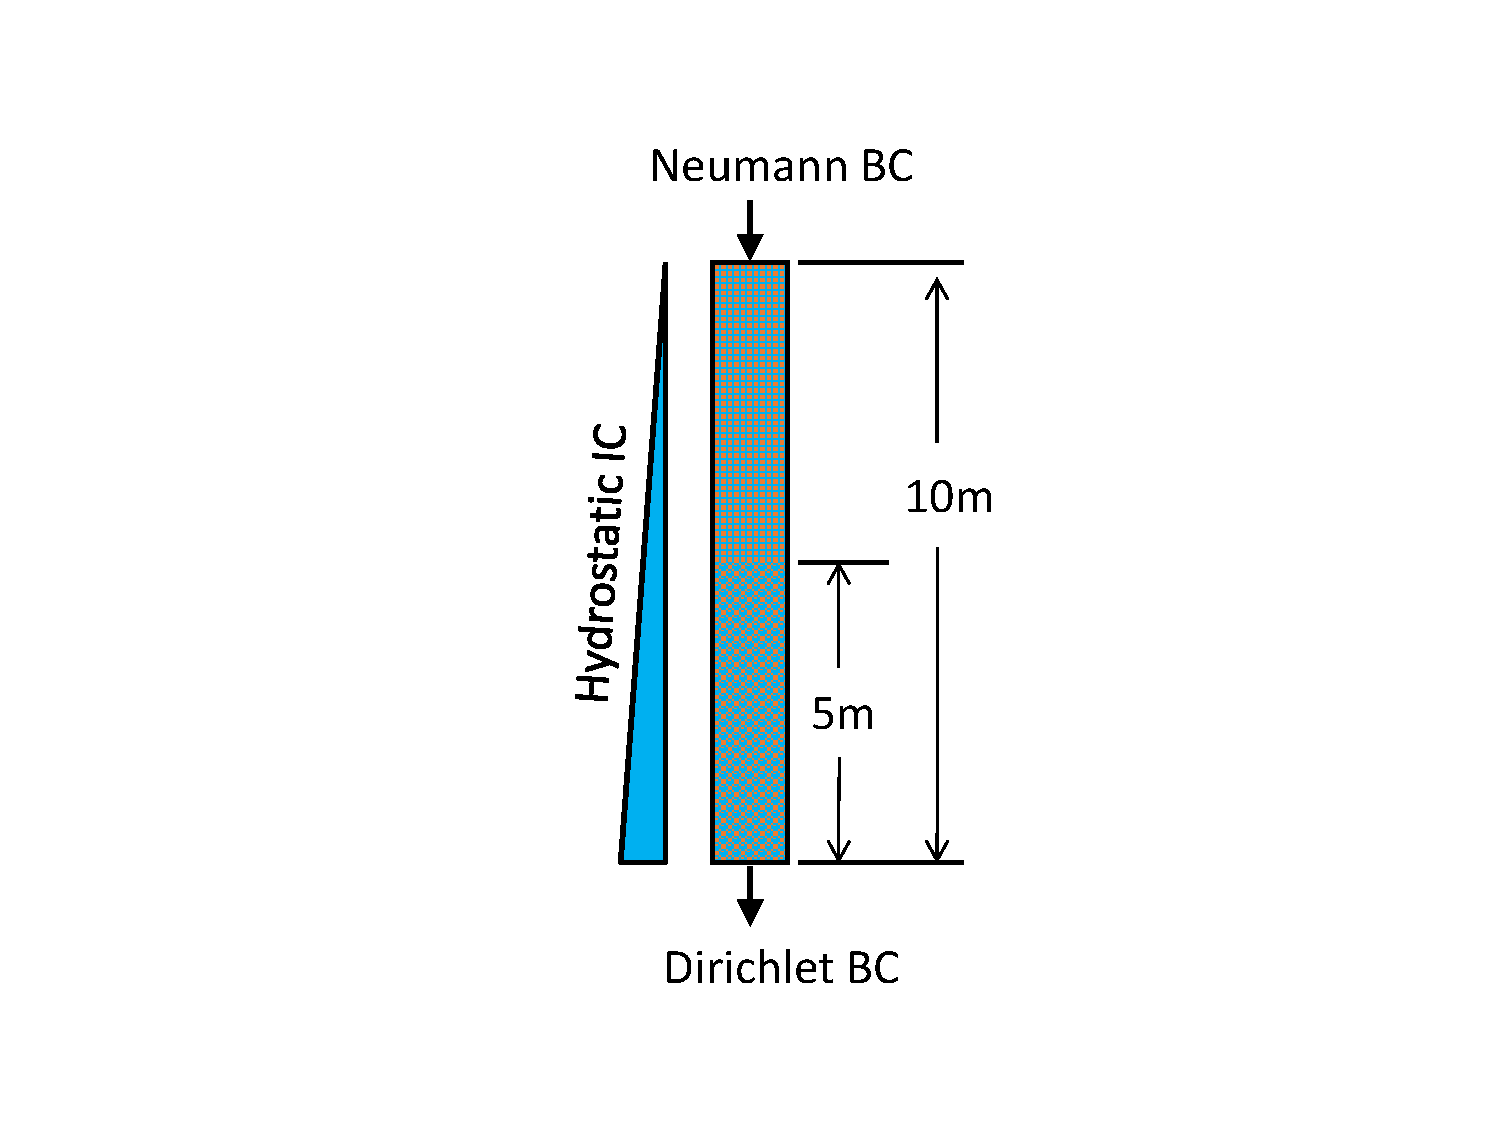
\includegraphics[height=2.5in]{./vsat_flow_layered}
\end{textblock} 
\end{frame}


%-----------------------------------------------------------------------------
\subsection{MATERIAL\_PROPERTY}

\begin{frame}[fragile]\frametitle{MATERIAL\_PROPERTY}

\begin{itemize}
\item Note the new porosity and permeability
\end{itemize}

\begin{semiverbatim}
\magentacomment{
MATERIAL_PROPERTY soil2    \bluecomment{! new soil name}
  ID 2                     \bluecomment{! new material ID}
  POROSITY 0.3d0
  PERMEABILITY
    PERM_ISO 2.d-12
  /
  CHARACTERISTIC\_CURVES cc2 \bluecomment{! new saturation function name}
END}
\end{semiverbatim}

\end{frame}

%-----------------------------------------------------------------------------
\subsection{CHARACTERISTIC\_CURVES}

\begin{frame}[fragile]\frametitle{CHARACTERISTIC\_CURVES}

\begin{itemize}
\item Note the new van Genuchten parameters
\end{itemize}

\begin{semiverbatim}
\magentacomment{
CHARACTERISTIC_CURVES cc2
  SATURATION_FUNCTION VAN_GENUCHTEN
    ALPHA 2.d-4
    M 0.6d0
    LIQUID_RESIDUAL_SATURATION 0.05d0
  /
  PERMEABILITY_FUNCTION MUALEM_VG_LIQ
    M 0.6d0
    LIQUID_RESIDUAL_SATURATION 0.05d0
  /
END}

\end{semiverbatim}

\end{frame}

%-----------------------------------------------------------------------------
\subsection{REGION}

\begin{frame}[fragile,containsverbatim,allowframebreaks]\frametitle{REGION}

\begin{itemize}
  \item Add regions defining top and bottom soil layers
  \item Add region defining a coordinate for an observation point
\end{itemize}

\begin{semiverbatim}


\magentacomment{
REGION top_layer
  COORDINATES
    0.d0 0.d0 5.d0
    1.d0 1.d0 10.d0
  /
END




REGION bottom_layer
  COORDINATES
    0.d0 0.d0 0.d0
    1.d0 1.d0 5.d0
  /
END

REGION middle    \bluecomment{! note the singular COORDINATE}
  COORDINATE 0.5d0 0.5d0 5.d0
END}

\end{semiverbatim}

\end{frame}

%-----------------------------------------------------------------------------
\subsection{STRATA}

\begin{frame}[fragile]\frametitle{STRATA}

\begin{itemize}
\item Change region for existing soil type
\item Add new strata coupling for new soil layer at bottom of domain
\end{itemize}

\begin{semiverbatim}

STRATA
  REGION \magentacomment{top_layer}
  MATERIAL soil1
END

\magentacomment{
STRATA
  REGION bottom_layer
  MATERIAL soil2
END}

\end{semiverbatim}

\end{frame}

%-----------------------------------------------------------------------------
\subsection{OBSERVATION}

\begin{frame}[fragile]\frametitle{OBSERVATION}

\begin{itemize}
\item Couples an observation point to a region
\end{itemize}

\begin{semiverbatim}

\magentacomment{
OBSERVATION
  REGION middle
  VELOCITY      \bluecomment{! print flow velocities}
END}

\end{semiverbatim}

\end{frame}

%-----------------------------------------------------------------------------
\subsection{OUTPUT}

\begin{frame}[fragile]\frametitle{OUTPUT}

\begin{itemize}
\item Change output times to 0.5 1. 2. 5. years
\item Add output of observation data at every time step
\end{itemize}


\begin{semiverbatim}

OUTPUT
  \magentacomment{TIMES y 0.5 1. 2. 5.}   
  \magentacomment{PERIODIC_OBSERVATION TIMESTEP 1} \bluecomment{! print observation}
  FORMAT TECPLOT POINT            \bluecomment{!   data every time step}
END

\end{semiverbatim}

\end{frame}

%-----------------------------------------------------------------------------
\subsection{TIME}

\begin{frame}[fragile]\frametitle{TIME}

\begin{itemize}
\item Change final simulation time to 35 years
\end{itemize}

\begin{semiverbatim}

TIME
  FINAL_TIME \magentacomment{35.d0} y
  INITIAL_TIMESTEP_SIZE 1.d0 h
  MAXIMUM_TIMESTEP_SIZE 5.d-2 y
END

\end{semiverbatim}

\end{frame}

%-----------------------------------------------------------------------------
\subsection{Running vsat_flow_pulse_2layer.in}

\begin{frame}[fragile]\frametitle{Running PFLOTRAN}

\begin{semiverbatim}

> cd $PFLOTRAN_DIR
> cd shortcourse/exercises/1D_variably_saturated_flow
> pflotran -input_prefix vsat_flow_pulse_2layer
> python vsat_flow_pulse_2layer.py
> python vsat_flow_pulse_2layer_obs.py
\end{semiverbatim}

\end{frame}

\end{document}
